
En el desarrollo teórico ideal se supuso que el comparador conmuta instantáneamente
cuando la señal triangular alcanza alguno de los umbrales del disparador Schmitt,
es decir, cuando llega a $V_{IL}$ o a $V_{IH}$ (ver Figura~\ref{fig:comparador-ideal}). Bajo esa hipótesis, el período de oscilación queda determinado únicamente por la pendiente de carga/descarga del
integrador y por la separación entre los umbrales.

\begin{figure}[H]
    \centering
    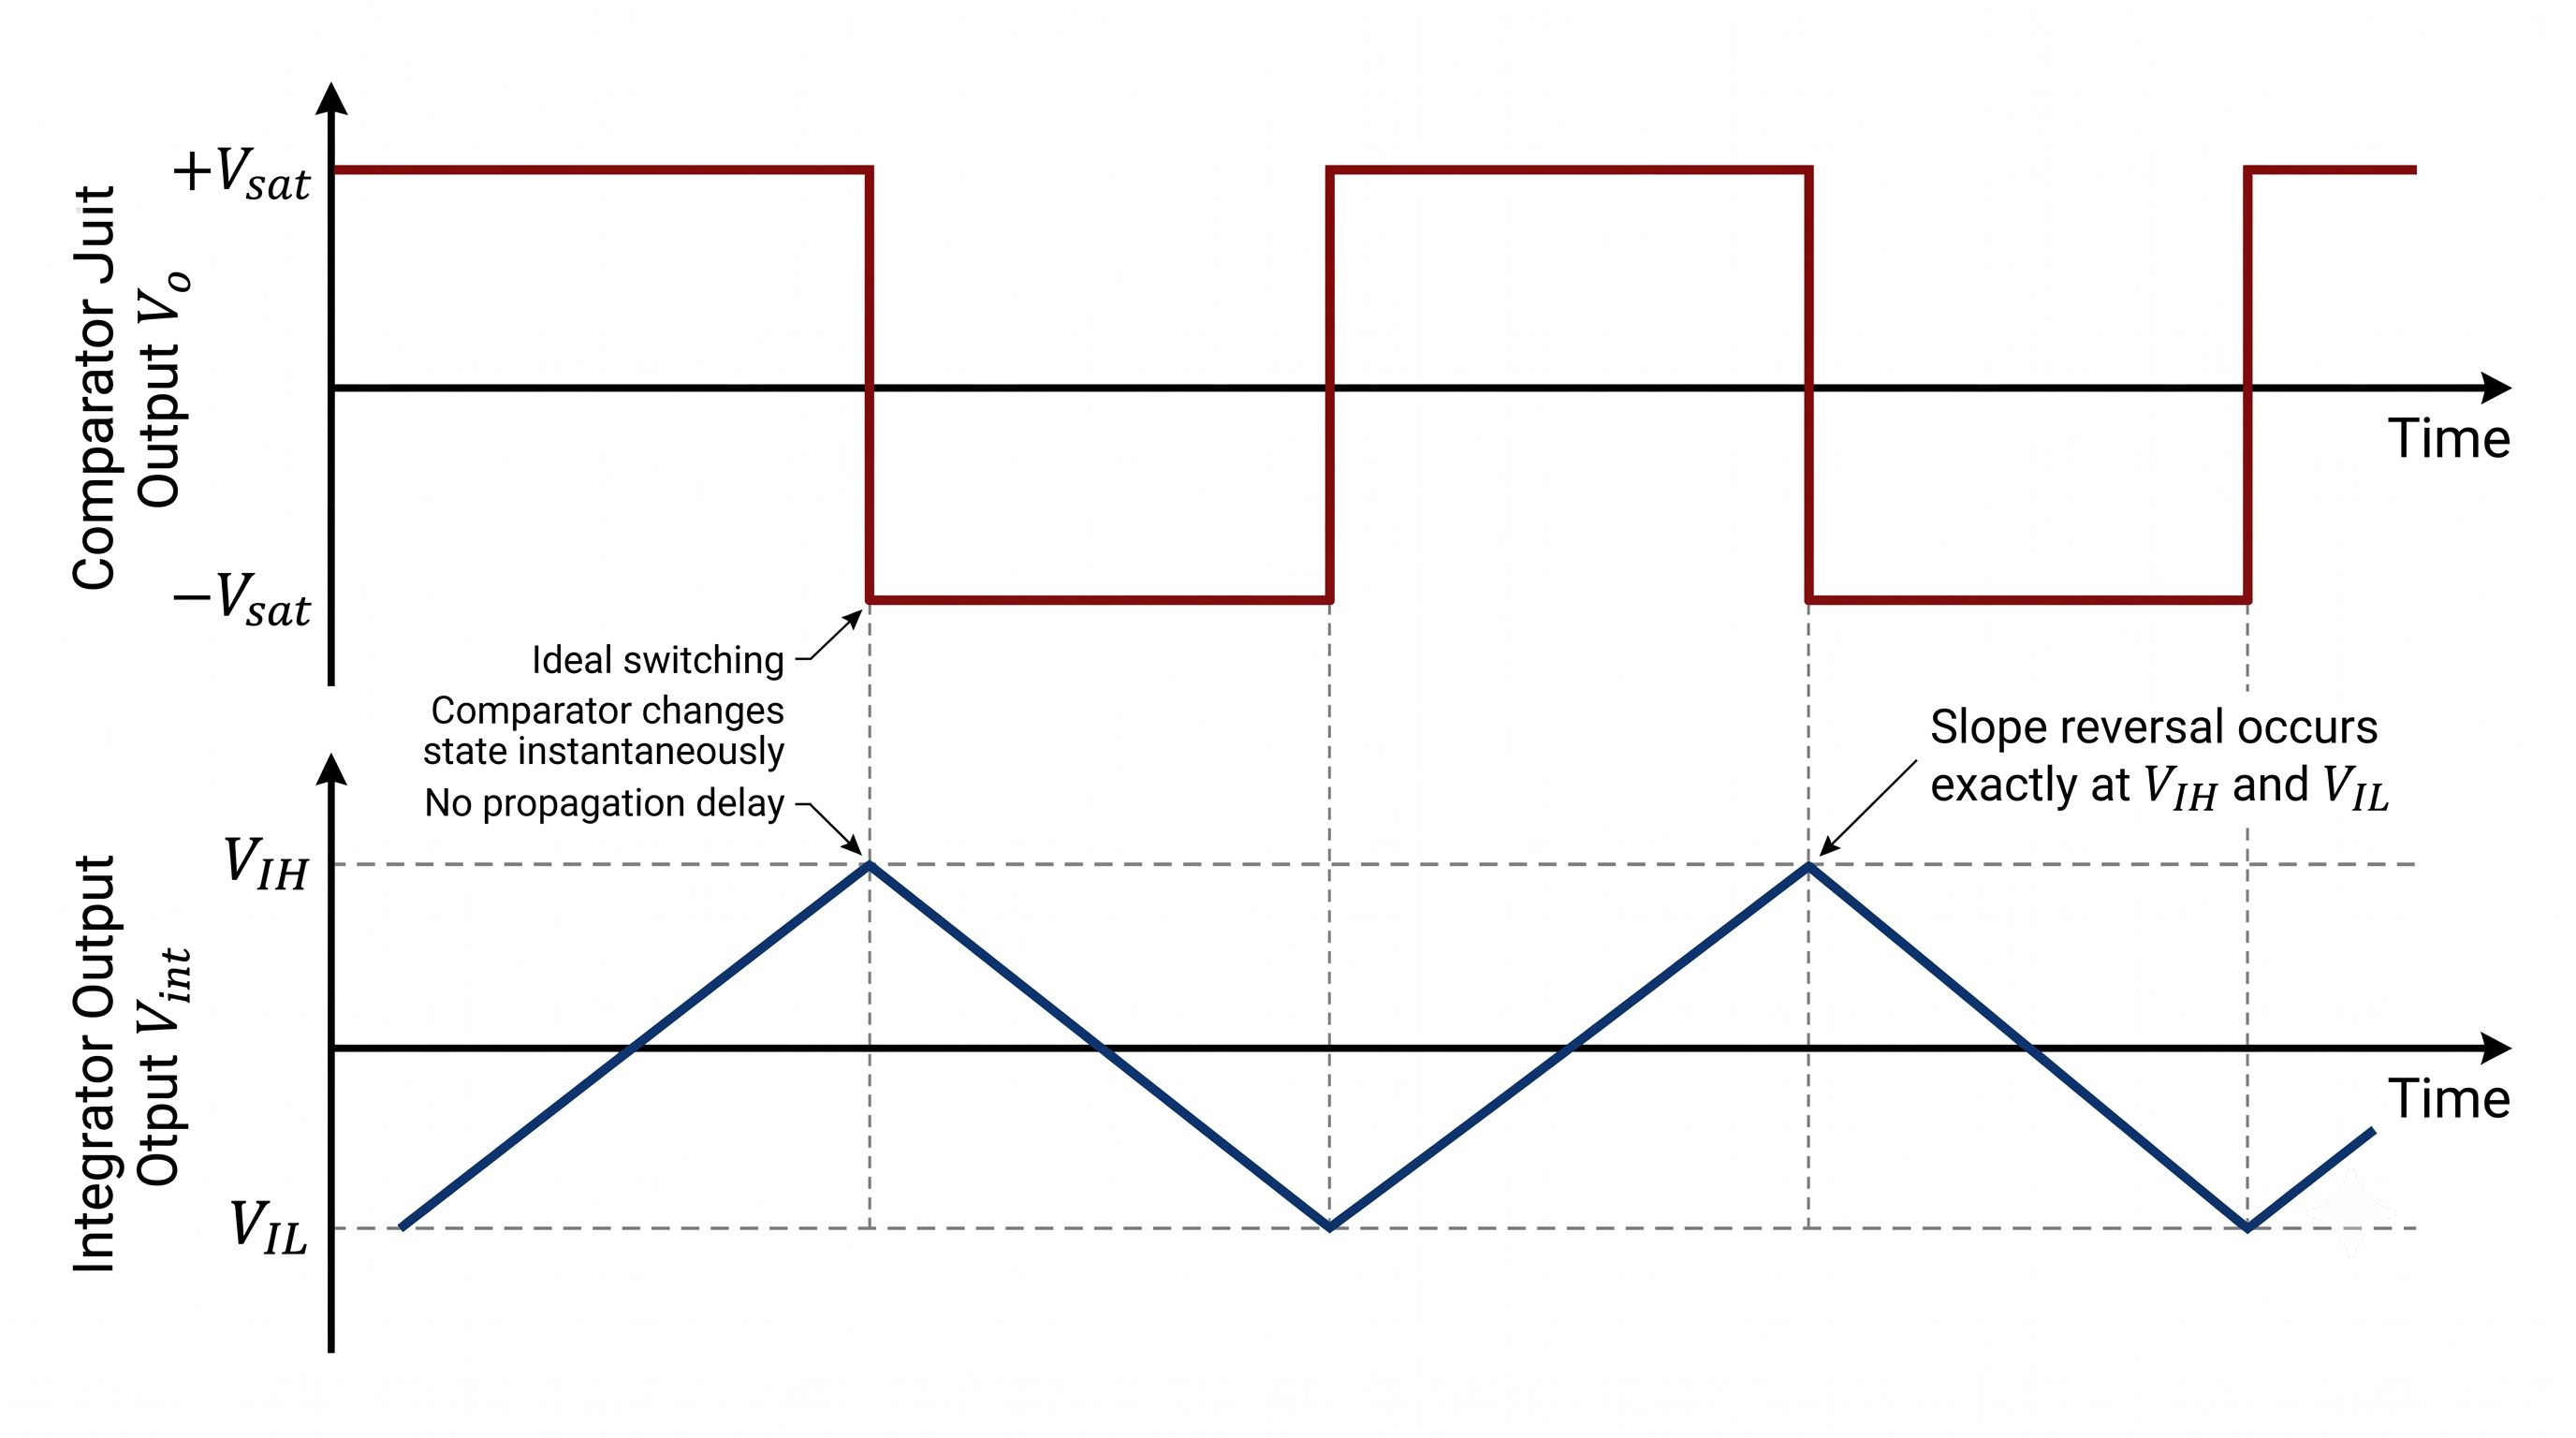
\includegraphics[width = 0.7\textwidth]{img/modif-pwm/comparador-ideal.png}
    \caption{Como se vería al commutar instanáneamente.}
    \label{fig:comparador-ideal}
\end{figure}

Para el circuito, la frecuencia ideal queda dada por
\begin{equation*}
    f_0 = \frac{1}{4RC}\frac{R_{f1}}{R_{f2}}\,.
\end{equation*}
O, equivalentemente, el período ideal es
\begin{equation*}
    T_0 = 4RC\frac{R_{f2}}{R_{f1}}\,,
\end{equation*}
donde, si se reemplaza con los valores obetenidos de resistencias y capacitor ($R_{f1}=\SI{560}{\kilo\ohm}$, $R_{f2}=\SI{56}{\kilo\ohm}$, $R=\SI{220}{\kilo\ohm}$ y $C=\SI{56}{\pico\farad}$) queda de la siquiente manera:
\begin{equation*}
    T_0 \approx \SI{4.93}{\micro\second} \, .
\end{equation*}


Por lo tanto,
\begin{equation*}
    f_0 = \frac{1}{T_0} \approx \SI{202.9}{\kilo\hertz} \, .
\end{equation*}

Este resultado corresponde al caso ideal, donde el tiempo de propagación del
comparador se considera nulo.

Sin embargo, en la medición se observa que la frecuencia de oscilación no es
$202,9\,\text{kHz}$, sino aproximadamente $f_{medida} \approx \SI{129.5}{\kilo\hertz}$.


Esto implica un período simulado de $T_{medido} = \frac{1}{f_{medida}} \approx 7,72\,\upmu$s.

La diferencia entre la frecuencia ideal y la observada se debe principalmente al
tiempo de propagación del comparador LM393. A partir de la medición de este tiempo de propagación con el osciloscopio se obtuvo
\begin{equation*}
    t_p \approx \SI{0.6}{\micro\second} \, .
\end{equation*}

Este tiempo se midió a partir de la observación de las entradas del comparador, la entrada roja es la $V_{ref}$, cuando la celeste supera a la tensión de referencia, la salida debería cambiar a $V_{CC}$, pero se observa que tarda un poco en realizar ese cambio (ver Figura~\ref{fig:tiempo-propagacion}).

\begin{figure}[H]
    \centering
    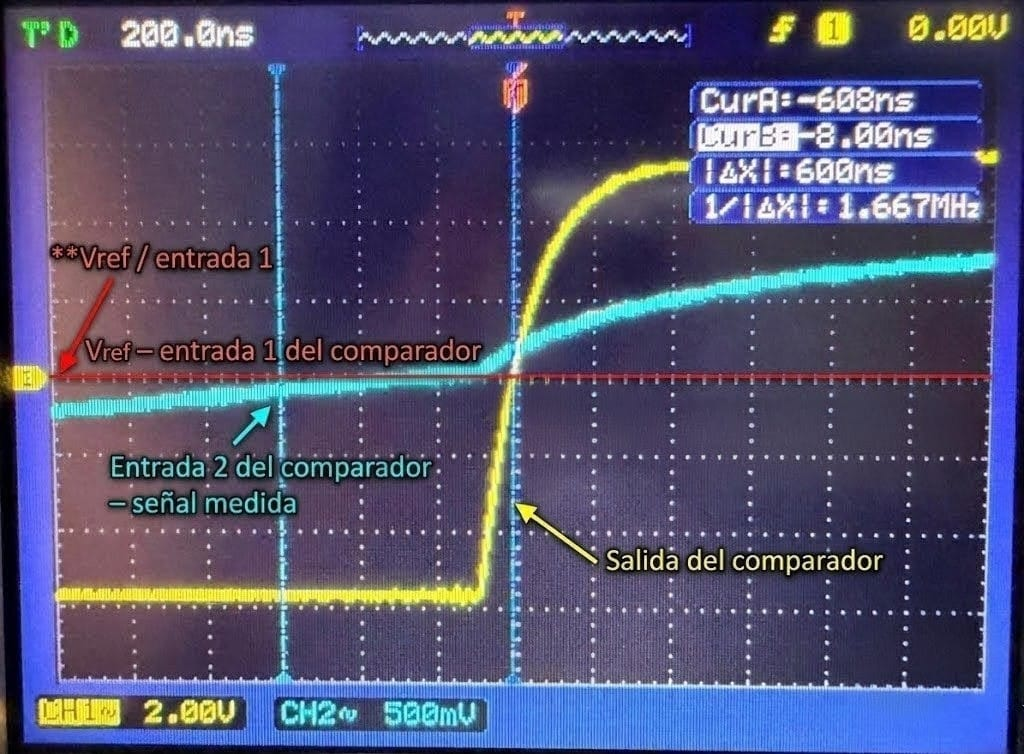
\includegraphics[width = 0.7\textwidth]{img/modif-pwm/tiempo-de-propagacion.jpeg}
    \caption{Tiempo de propagación del comparador LM393 medido con el osciloscopio.}
    \label{fig:tiempo-propagacion}
\end{figure}

La idea importante es que el comparador no cambia su salida exactamente en el
instante en que la señal cruza el umbral de $V_\text{REF}$. La salida del comparador recién conmuta un tiempo $t_p$ después. Durante ese intervalo, el integrador sigue integrando en el mismo sentido.

Por ejemplo, si la triangular está bajando y cruza $V_{IL}$, el comparador
debería cambiar su salida en ese instante. Pero como existe un retardo $t_p$, la
salida todavía no cambia y el integrador sigue haciendo bajar la triangular.
Entonces la señal no se detiene en $V_{IL}$, sino que se pasa por debajo de ese
valor. Lo mismo ocurre cuando la triangular sube y cruza $V_{IH}$: durante el
tiempo de propagación, sigue subiendo y se pasa por encima del umbral.

Ese sobrepaso puede estimarse como: $\Delta V_{over} = m \cdot t_p.$

Donde $m$ es la pendiente de la señal triangular. En este caso, como el
circuito está centrado alrededor de $V_\text{REF}$ y las pendientes de subida y bajada
son aproximadamente iguales, se puede estimar
\begin{equation*}
    m \approx \frac{V_{CC}/2}{RC} \, .
\end{equation*}

Tomando $V_{CC}=\SI{9.1}{\volt}$, se obtiene una pendiente $m \approx 0,369\frac{\text{V}}{\upmu\text{s}}$.

Entonces, para $t_p = \SI{0.6}{\micro\second}$, se obtiene una $\Delta V_{over} \approx \SI{0.22}{\volt}$.

Este valor no es despreciable frente a la histéresis ideal del disparador
Schmitt. La diferencia ideal entre los umbrales es aproximadamente
\begin{equation*}
    V_{IH}-V_{IL} \approx \frac{R_{f2}}{R_{f1}}V_{CC}\,;
\end{equation*}
\begin{equation*}
    V_{IH}-V_{IL} \approx \SI{0.91}{\volt} \, .
\end{equation*}

Pero por el tiempo de propagación, la triangular se pasa aproximadamente
$\SI{0.22}{\volt}$ en cada extremo. Por lo tanto, la excursión efectiva de la triangular
ya no es solamente $\SI{0.91}{\volt}$, sino

\begin{equation*}
    \Delta V_{eff} \approx 0.91\,\text{V} + 2 \cdot 0.22\,\text{V}\,,
\end{equation*}

\begin{equation*}
    \Delta V_{eff} \approx 1.35V\,.
\end{equation*}

Es decir, el tiempo de propagación hace que la triangular tenga que recorrer una
excursión mayor. Como la pendiente del integrador es prácticamente la misma, si
la señal tiene que recorrer más tensión, tarda más tiempo. Por eso aumenta el
período y baja la frecuencia.

Entonces, por cada conmutación, el retardo efectivo agregado al período es
aproximadamente:

\begin{equation*}
    t_p + t_p = 2t_p
\end{equation*}

Como en un período completo hay dos conmutaciones, una en $V_{IL}$ y otra en
$V_{IH}$, la corrección total queda:

\begin{equation*}
    T \approx T_0 + 4t_p
\end{equation*}

Reemplazando: $T \approx \SI{7.33}{\micro\second}$. Y, por lo tanto, la frecuencia queda: $f \approx 136.5kHz$.

Este valor se acerca mucho más al resultado de la medición, $f_{medida} \approx 129.5kHz$.

La diferencia restante puede explicarse porque el modelo real del comparador no
se comporta como un retardo ideal puro. Además del tiempo de propagación, pueden influir también efectos no ideales, como los tiempos de subida y bajada, posibles diferencias entre el retardo de flanco ascendente y descendente, entre otros.

Por lo tanto, la diferencia entre la frecuencia teórica ideal y la frecuencia
simulada se debe a que el tiempo de propagación del comparador no es despreciable
frente al período de oscilación. En nuestro caso:

\begin{equation*}
    \frac{t_p}{T_0} \approx \frac{\SI{0.6}{\micro\second}}{\SI{4.93}{\micro\second}} \approx 0.12
\end{equation*}

Es decir, el tiempo de propagación representa aproximadamente un $12\%$ del
período ideal. Y, como su efecto aparece aproximadamente cuatro veces por
período, el error total sobre el período es mucho mayor a este.

Para que el tiempo de propagación pudiera despreciarse y producir un error menor
al $10\%$ en el período, debería cumplirse aproximadamente:

\begin{equation*}
    4t_p < 0.1T_0
\end{equation*}

\begin{equation*}
    t_p < 0.025T_0
\end{equation*}

Como $T_0 \approx 4.93\mu s$:

\begin{equation}
    t_p < 0.123\mu s
\end{equation}

Mientras que el tiempo de propagación observado es de aproximadamente
$\SI{0.6}{\micro\second}$, bastante mayor que ese valor. Por lo tanto, no puede despreciarse.
